\section{Audio Preprocessing}
TODO: rewrite this with more details.

Audio preprocessing is an essential step in preparing collected audio data for use in machine learning models. The preprocessing techniques involve noise reduction, feature extraction, analysis, and selection. This section discusses important aspects of audio preprocessing, including noise reduction and audio trimming.

\subsection{Noise Reduction}

One common strategy for denoising music is spectral gating, which involves gating the signal only on high-level sounds. Non-stationary noise reduction is an extension of stationary noise reduction that allows the noise gate to change over time. In this method, a spectrogram is calculated over the signal, and a time-smoothed version of the spectrogram is computed using an IIR filter applied forward and backward on each frequency channel. A mask is computed based on the time-smoothed spectrogram, which is then smoothed with a filter over frequency and time. The mask is applied to the spectrogram of the signal and then inverted.

To implement these noise reduction techniques, we recurred to the "noisereduce" library. This algorithm relies on the spectral gating method and estimates a noise threshold for each frequency band of the signal/noise. This threshold is used to compute a mask, which gates noise below the frequency-varying threshold. The Code Snippet \ref{nr:code} shows how we implemented the noise reduction technique.

\begin{listing}[H]
	\begin{minted}{python}
		noisereduce.reduce_noise(
		y=y, sr=16000, n_fft=2048, hop_length=512, prop_decrease=.75, time_constant_s=1
		)
	\end{minted}
	\caption{Python code for applying noise reduction using the noisereduce library}
	\label{nr:code}
\end{listing}


\subsection{Audio Trim}

Trimming silence at the beginning and end of audio files is another important preprocessing step. By removing the silence from audio files, the resulting audio data will be more focused on the relevant audio content and will be easier to process by machine learning algorithms.

Upon visually observing several wave plots we ended up considering 30 decibels or lower as silence and trimmed every audio file at the beginning and end of each audio.


\begin{figure}[H]
	\centering
	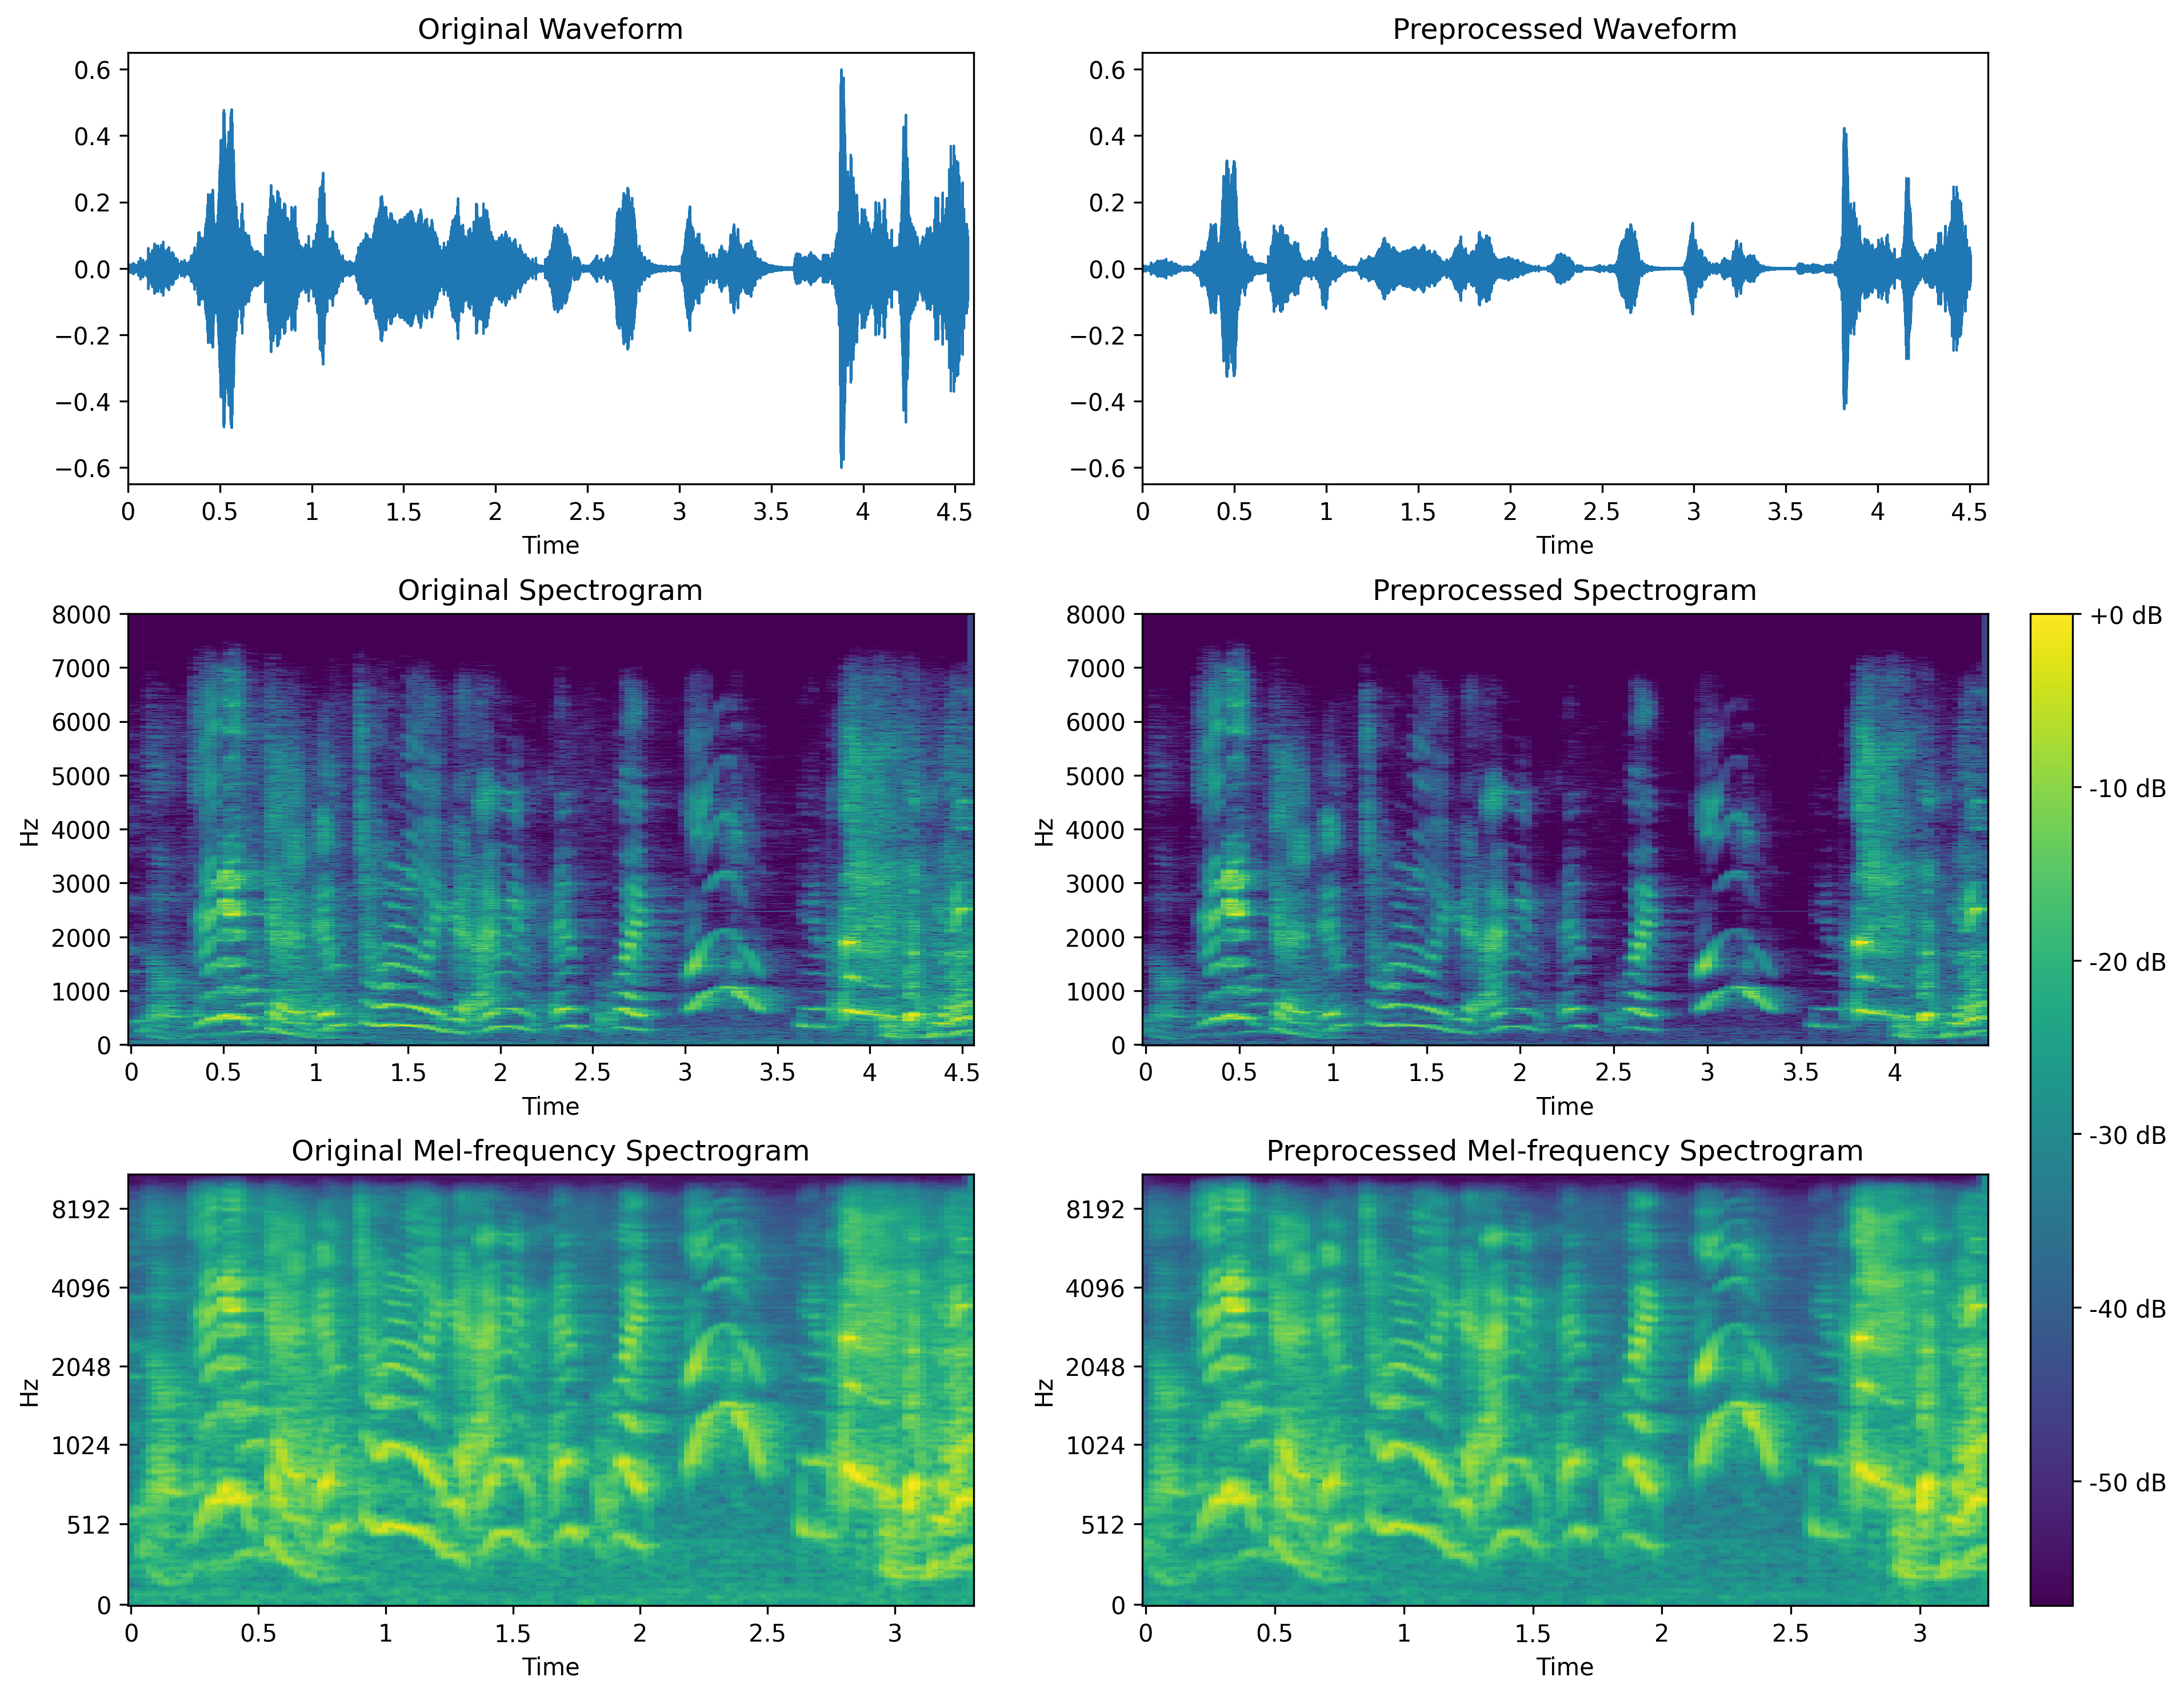
\includegraphics[width=\textwidth]{figs/4_2_preprocessing/preprocessing.png}
	\caption{Visual representations of audio features before and after preprocessing.}
	\label{fig:prep}
\end{figure}

